\section{Algorithm}

\begin{frame}[t]{Getting started}
    \framesubtitle{What do we need?}
	
    \vspace{0.5cm}
    \begin{itemize}
    \item<+->{
        \stress{Quantify \enquote{similar}} {\color{purple}(\emph{metric})}:\\
    	$\lra$ Similarity test\\
        $\phantom{\lra}$ {\small e.g. $\chi^2$ test, Kolmogorov test, \dots}
	}
    
    \item<+->{
    	\bigskip
    	\stress{Build up groups} {\color{purple}(\emph{clusters})} of similar distributions:\\
    	$\lra$ Clustering algorithm\\
        $\phantom{\lra}$ {\small e.g. Hierarchical clustering, \dots}
    }
    
    \item<+->{
        \bigskip
        \stress{Select representatives} {\color{purple}(\emph{benchmark points})} from each cluster
    }
    
    \item<+->{
    	\bigskip
    	\stress{How many} clusters do we want?\\
    	$\lra$ Add experimental error expectation\\
    	$\lra$ Keep as many clusters as we can distinguish
    }
    \end{itemize}
\end{frame}

\begin{frame}{The metric}{Similarity between distributions}
	\begin{itemize}
		\item Let's take two points in parameter space and their corresponding kinematic histograms \hhl{$H_{1,2}$} with bin contents \hhl{$n_{1i}$}
		\item How well would we be able to distinguish between both cases?
		\item Estimate experimental uncertainties when conducting measurement \srem{(under the assumption that $H_k$ is the truth distribution)} $\lra$ Covariance matrices \hhl{$\Sigma_{1,2}$} 
		\item Let's assume that the measurement would indeed return the expectation value $H_{1,2}$ with $\Sigma_{1,2}$
		\item Use a test statistic that allows to include uncertainties 
		\item In the paper we only compared the shape of the histograms $\lra$ test statistic shouldn't depend on normalization
		\item Used a \hhl{$\chi^2$ test with normalization} \srem{(and made some mistakes in the paper)}	
	\end{itemize}
\end{frame}

\begin{frame}{The metric}{$\chi^2$ metric}
	\begin{itemize}
		\item Slide about different formulas for $\chi^2$
		\item Correct mistake about dofs
		\item With and without correlation
	\end{itemize}
\end{frame}

\begin{frame}{The metric}{Slight tangent: Normalized $\chi^2$ metric can be dangerous}
	
\end{frame}

\begin{frame}{The metric}{Validation}
	
\end{frame}

\begin{frame}[t]{Example: Hierarchical Clustering}
	\vspace{0.5cm}
   \centering
	\only<+>{
		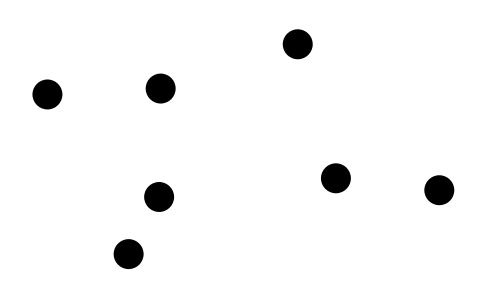
\includegraphics[width=10cm]{figures/hierarchy/step0.pdf}\\[2ex]
		Step 0: 7 points in the parameter space
	}
	\only<+>{
		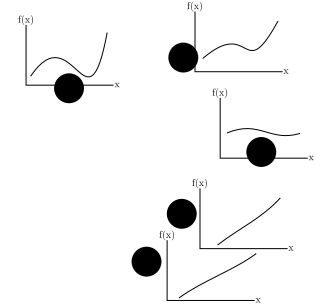
\includegraphics[width=10cm]{figures/hierarchy/step0_curves.pdf}\\[2ex]
		Step 0: 7 points in the parameter space = 7 distributions
	}
	\only<+>{
		\includegraphics[width=10cm]{figures/hierarchy/step1_curves.pdf}\\[2ex]
		Step 1: Every point is its own cluster
	}
	\only<+>{
		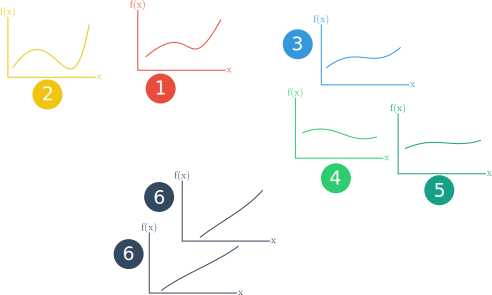
\includegraphics[width=10cm]{figures/hierarchy/step2_curves.pdf}\\[2ex]
		Step 1: Distributions from cluster 6 and 7 were the most similar $\Lra$ Merged!
	}
	\only<+>{
		\includegraphics[width=10cm]{figures/hierarchy/step3_curves.pdf}\\[2ex]
		Step 1: Cluster 4 and 5 were the next most similar clusters $\Lra$ Merged!
	}
	\only<+>{
		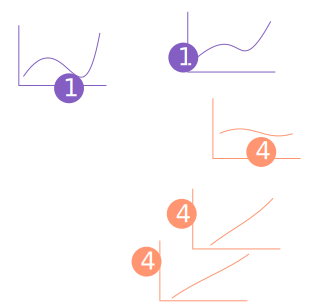
\includegraphics[width=10cm]{figures/hierarchy/step4_curves.pdf}\\[2ex]
		Step 1: 4 clusters remaining
	}
	\only<+>{
		\includegraphics[width=10cm]{figures/hierarchy/step5_curves.pdf}\\[2ex]
		Step 1: 3 clusters remaining
	}
	\only<+>{
		\includegraphics[width=10cm]{figures/hierarchy/step6_curves.pdf}\\[2ex]
		Step 1: 2 clusters remaining
	}
	\only<+>{
		\includegraphics[width=10cm]{figures/hierarchy/step7_curves.pdf}\\[2ex]
		Step 1: 1 cluster remaining
	}
	
%	}
\end{frame}